% umbenennen in Forschungsstand??
\chapter{Forschungsstand}
\label{chap:forschungsstand}
Seit den Anfängen der Entwicklung von \gls{open-ran} im Februar 2016 und der Gründung von \gls{oran} 2018 gibt es einige wissenschaftliche Arbeiten, die sich mit dem Thema Sicherheitsanalyse und Schwachstellenbewertung in einer \gls{open-ran} Umgebung beschäftigen. In diesem Kapitel wird ein Überblick über den Forschungsstand anhand einer Auswahl von Arbeiten gegeben \cite{Us} \autocite{GuideOpenRAN}.
\section{O-RAN Security Threat Modeling and Risk Assessment}
Die \gls{wg11} der \gls{oran} beschäftigt sich mit den sicherheitstechnischen Aspekten von \gls{open-ran} und veröffentlicht in regelmäßigen Abständen einen technischen Report, der eine Bedrohungsmodellierung und Risikobeurteilung enthält.
Zum Zeitpunkt der Veröffentlichung ist der Report in Version \textit{\textsf{v04.00}} die neuste Fassung dieses Dokuments.
Der Report umfasst sowohl mögliche Angriffe auf Komponenten in einem \gls{oran}-System, als auch nicht \gls{oran} spezifische Bedrohungen, wie Supply-Chain-Angriffe auf Quell-Offenen Programmcode oder physischen Eingriff um auf sensible Daten zu erlangen\autocite{o-ranworkgroup11securityworkgroupORANSecurityThreat2024}.
Der Einfachheit halber wird im Folgenden nur auf die \gls{oran}-spezifischen Bedrohungen eingegangen. Die betroffenen Komponenten sind in Abbildung \ref{fig:oran-components} dargestellt.
Die \gls{wg11} identifiziert dazu 35 Bedrohungen in der Komponente \textit{O-RAN Cloud} und 69 Bedrohungen die auf alle anderen Komponenten zutreffen \autocite[Seite 31 - 69]{o-ranworkgroup11securityworkgroupORANSecurityThreat2024}.

Der Großteil der Bedrohungen wird dabei in der Risikobewertung mit einem Risikowert von \textit{High} eingestuft, vgl. Abbildung \ref{fig:riskscore-oran-components} \autocite[Seite 130 - 164]{o-ranworkgroup11securityworkgroupORANSecurityThreat2024}.

\begin{figure}
    \centering
    \label{fig:riskscore-oran-components}
    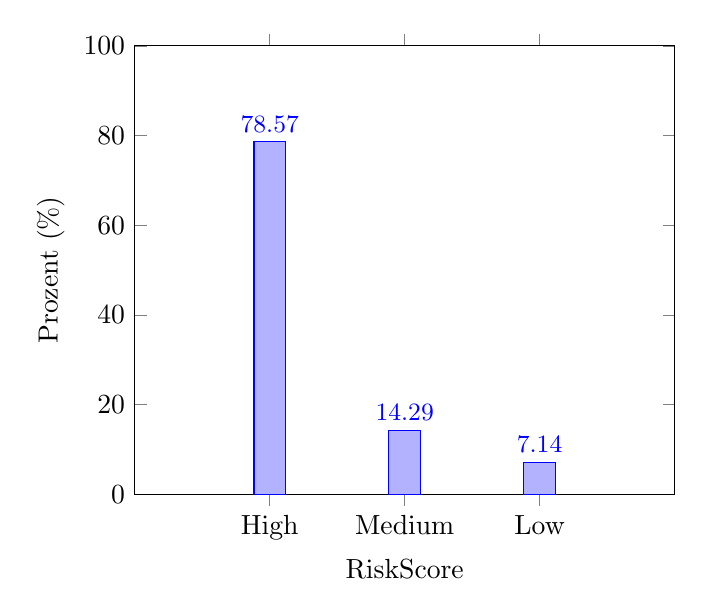
\begin{tikzpicture}
        \begin{axis}[
            ybar,
            symbolic x coords={High, Medium, Low},
            xtick=data,
            ymin=0, ymax=100,
            ylabel={Prozent (\%)},
            xlabel={RiskScore},
            nodes near coords,
            every node near coord/.append style={font=\small},
            bar width=0.4cm,
            enlarge x limits=0.5
        ]
            \addplot coordinates {(High, 78.57) (Medium, 14.29) (Low, 7.14)};
        \end{axis}
    \end{tikzpicture}
    \caption{Risikobewertung der Bedrohungen in der O-RAN Komponenten}
\end{figure}



